\begin{savequote}[75mm]
We are so familiar with seeing, that it takes a leap of imagination to realize that there are problems to be solved. But consider it. We are given tiny distorted upside-down images in the eyes, and we see separate solid objects in surrounding space. From the patterns of stimulation on the retina we perceive the world of objects and this is nothing short of a miracle.
\qauthor{Richard L. Gregory, \textit{Eye and Brain}, 1966.}
\end{savequote}

%Human knowledge is built on a few foundational domains, such as space, time, objects, action, causality ... (Piaget and Inhelder 1967, Minksy 1975)

%Spatial knowledge is the most fundamental of these (Lakoff and Johnson 1980).

\chapter{Introduction}
\lettrine[lines=3, loversize=0.3]{\textcolor{DarkBlue}T}he human visual cortex is able to process a bewilderingly large amount of data with ease. From messy signals emitted by the 100 million rods and cones in a typical retina, it can assemble an ordered world containing structure, meaningful parts, and distinct objects \cite{kandel2000principles}. Furthermore, it possesses an understanding of coherent motion, allowing it to keep track of and intuitively predict object trajectories. These two abilities, the segmentation of the world into objects, and the tracking of objects to maintain their identities, serve as key components in the bootstrapping of higher level knowledge. Indeed, it has been shown that our earliest and most fundamental understanding of the world is topological in nature, dealing with concepts that can be described through segmentation and tracking - proximity, order, separation and enclosure\cite{piaget1967}.

In fact, these concepts are so fundamental to human understanding of the world that we find it profoundly difficult to precisely define what an object actually is. Yet in spite of the difficulty in formalizing the concept, we can divide complex moving scenes into distinct objects, even hierarchies of parts, with little effort. In this work we argue that the concepts of tracking and segmentation are inexorably linked; that visual tracking plays an essential role in creating the objects we observe, and that the organization of observations into structured objects is critical for robust tracking. We propose that without the ability to track motions in a coherent way, the notion of distinct objects is, ultimately, a meaningless one. Furthermore, we suggest that this link between tracking and object segmentation is one of the key elements that enable learning from visual input, and through this, the bootstrapping of cognition itself.

\section{Problem Definition and Motivation}
As with humans, in order for intelligent agents to be truly autonomous, they must be able to learn the principles of visual understanding from their own unsupervised observations. At its most basic level, an agent must be able to parse observations, to break them down into meaningful entities upon which higher level knowledge can be built. In other words, segmentation of observations is a precursor to high-level behaviors, such as identification of objects, scene understanding, and task planning. Tracking segmented entities over time is an integral parts of this, as it further enriches this knowledge by extending it to the action domain. Combining these two tasks - segmentation and tracking - would allow fully unsupervised parsing of streaming visual data.   This has the potential to greatly increase the flexibility of autonomous robotic systems by allowing them to learn from observations without the constraints of pre-defined object and domain knowledge.

In this work, we propose to develop an unconstrained video segmentation algorithm that is able to track low level patches. This permits the segmentation of objects and their parts naturally, without the need to define what an object actually is. Rather than train classifiers to recognize pre-defined objects, we can have an agent observe or interact with a scene and learn the concept of an object through movement and interactions between observed patches. This Chapter introduces the general concepts that will be expounded upon throughout the work by first discussing the three underlying tasks; Image Segmentation, \acrfull{mtt}, and \acrfull{vos}. With each of these tasks, we will discuss what exactly our goals are, and what challenges are faced in achieving them. Next, we survey the state of the art in each of these fields, highlighting the methods and important papers upon which we base this work. Finally, we outline each of the Chapters of this work, and enumerate the specific contributions of our research.

\subsection{The Image Segmentation Problem}
Image segmentation aims to divide the set of pixels in an image into a number of distinct subsets, where each subset represents some semantically meaningful entity (e.g., an object - see Figure \ref{ExampleSeg}). This is a (infamously) deceptively tricky business, primarily because it is something that humans are able to do intuitively. This ease with which humans can segment visual scenes is highly deceptive; Marvin Minsky, one of the pioneers of \gls{ai}, famously assigned one of his students ``computer vision'' as a summer undergraduate project in 1966. Nearly half a century later, despite the extensive effort to solve it, image segmentation, the first step on the long road to complete ``computer vision'', remains an unsolved problem.  In fact, this phenomenon - of tasks that are simple for humans being incredibly demanding computationally - even has its own name; \emph{Moravec's Paradox}. As stated by Pinker \cite{Pinker_Language}:

\begin{figure}[!t]
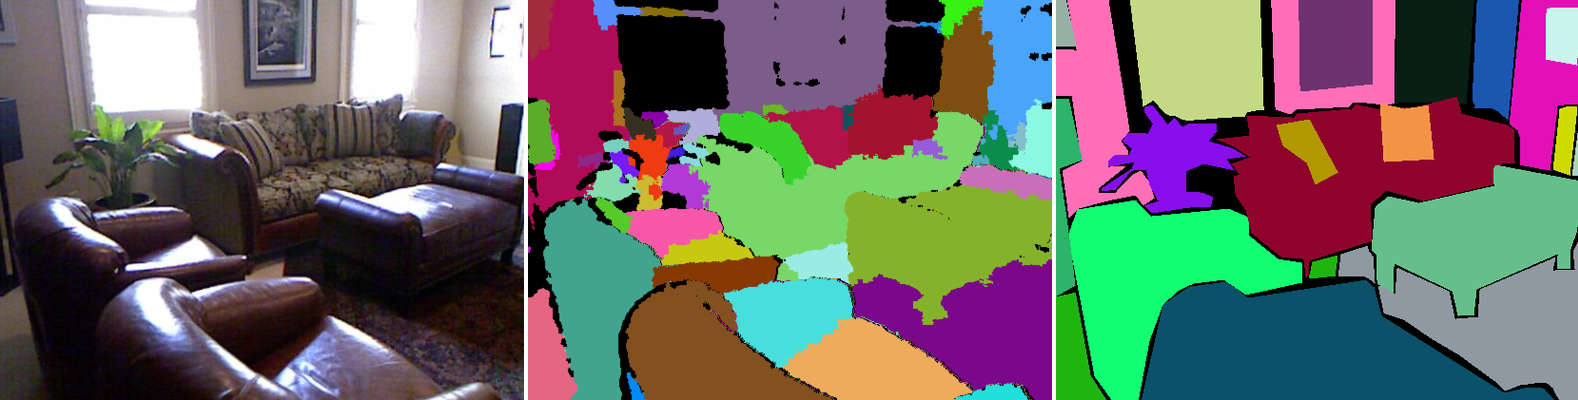
\includegraphics[width=\linewidth]{figures/Introduction/segmentation_GT_example.png}
\caption[Example of Segmentation and Ground Truth]{Example of Segmentation and one interpretation of Ground Truth. From left to right we have an image, a segmentation from a computer vision algorithm, and a human-annotated ground truth labeling. Here labels are represented by different colors, a convention we shall use throughout the rest of this work.}
\label{ExampleSeg}
\end{figure}

\begin{quote}
``The main lesson of thirty-five years of AI research is that the hard problems are easy and the easy problems are hard. The mental abilities of a four-year-old that we take for granted – recognizing a face, lifting a pencil, walking across a room, answering a question – in fact solve some of the hardest engineering problems ever conceived. (p. 190)''
\end{quote}

The reason for this ``hardness'' of an ``easy'' problem like image segmentation is two-fold: firstly, there are many technical and computationally-demanding challenges associated with properly dividing an image into separate objects. Among these, shadows, occlusions, reflections, imaging noise and so forth can all greatly affect the results of image segmentation. Consider, for instance, a partial occlusion as in Figure \ref{fig:SegmentationProblems}. A human can easily identify that the parts on either side of the occluding object belong to same object. This is accomplished using what we shall refer to as \emph{high-level} knowledge throughout this work - in this case, knowledge of the complete nature of an object.

This leads us to the second challenge in image segmentation, which is that, generally speaking, there is no ``correct'' solution to the problem. A perfect labeling for one application might be useless in another. This is even more of a problem when we are discussing segmentation separate from any application, as is the case with standard image segmentation benchmarks (which are use to quantify algorithm performance). These benchmarks use ground-truth image labels (manually created by humans) to score the output of different algorithms. Unfortunately, the correctness of different labellings is highly subjective, and hand-drawn labels from  people can differ radically.

\begin{figure}
\centering
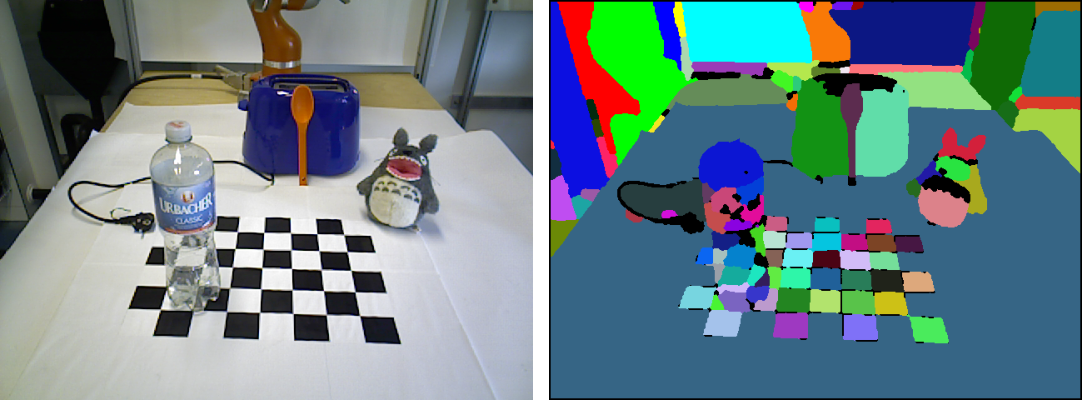
\includegraphics[width=\linewidth]{figures/Introduction/Segmentation_Problems.pdf}
\caption[Technical Difficulties of Segmentation]{Technical Difficulties of Segmentation. Here we see some of the myriad of technical difficulties present in color-based segmentation, such as transparent objects (the water bottle), partial occlusions (the toaster), objects with strong color differences (the little monster), and similarities in color (the bottle cap to the table).}
\label{fig:SegmentationProblems}
\end{figure}


\subsection{The Tracking Problem}
Tracking entities over time is a critical element in a wide variety of computer vision applications such as visual surveillance, action recognition, and robotic imitation learning. In most of these, visual tracking serves as the precursor to further high-level inference, as without it, one is unable to correctly interpret time-variant systems. One can formalize the tracking problem as estimation of the time-varying hidden state (e.g., position, velocity) of an object $x(t)$ using noisy observations $y(t)$. For simplicity, one generally assumes the state evolution to be a \emph{Markov Process} (see Figure \ref{fig:HMM}), that is, a stochastic process which is conditionally independent of the rest of its history given its previous state.    

\begin{figure}
\centering
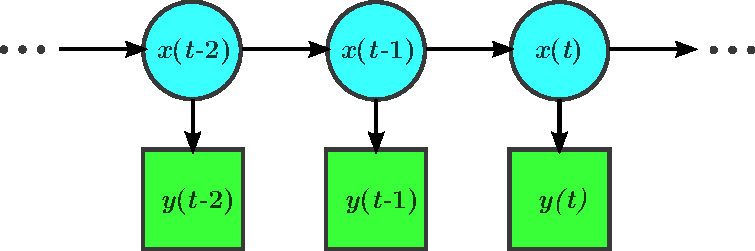
\includegraphics[width=0.9\linewidth]{figures/Introduction/HMM.pdf}
\caption[Hidden Markov Model]{The Hidden Markov Model is a classical way to represent the track of an object over time. The object states $x(0\dots t)$ (shown here in blue) are hidden variables which influence observations $y(0\dots t)$ through conditional dependencies (shown as arrows). An important property of the Markov Model is that state at time $t$ is dependent only on state at time $t-1$.}
\label{fig:HMM}
\end{figure}

\gls{mtvt} extends these concepts to multiple targets, adding additional complexity due to the need to both estimate the number of tracked targets as well as associate observations with appropriate targets. This is the primary challenge of \gls{mtvt} - the data association problem - deciding which tracked target a particular observation belongs to. Confounding this is the additional null possibility, where an observation belongs to none of the tracked targets. Some additional difficulties present in \gls{mtvt} are related to those of image segmentation, simply extended into the temporal domain. In particular, interacting and occluded targets are especially challenging.

\begin{figure}
\label{fig:ExampleTracking}
\centering
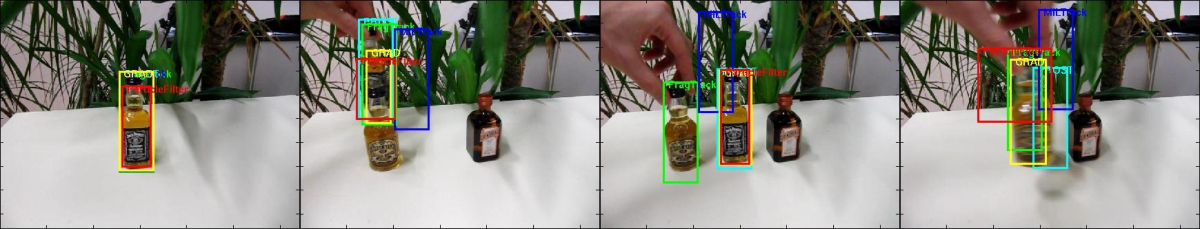
\includegraphics[width=\linewidth]{figures/Introduction/Tracking_Example.pdf}
\caption[Example of Visual Tracking]{Example of Visual Tracking - from \cite{PartFilter_Papon_2012}. This shows outputs from various trackers in a standard video tracking benchmark \cite{PROST}. The output of each tracker is shown as a colored rectangle. Some of the difficulties of tracking can be seen- in particular complex backgrounds, motion blur, partial occlusions (second frame from left) and even full occlusions (right-most frame).}
\end{figure}

\subsection{Video Object Segmentation - Segmentation In Sequential Frames}
\gls{vos} attempts to cluster pixels of video frames into segments which are both spatially and temporally coherent. While related to \gls{mtvt}, \gls{vos} goes a step beyond localizing tracked objects, in that it makes an association decision for each observed pixel; in addition to estimating overall state, it must re-estimate spatial extent every frame. Additionally, \gls{vos} has the additional consideration that target appearance models are unknown a-priori, and are subject to arbitrary changes over time. 

The standard interpretation of \gls{vos} is that of adding an additional dimension to image segmentation; that is, one stacks all the image frames on top of each other, and performs a ``volumetric'' segmentation. In this work we shall use a different interpretation for \gls{vos}; that of tracking multiple time-evolving and interacting objects projected onto the image plane of our sensor. While the standard interpretation has the advantage of allowing the straightforward extension of 2D segmentation techniques, it suffers greatly from its inability to handle occlusions in a meaningful way. This is easily observed when one considers that occlusions will result in ``disconnection'' within the 3D stack, violating the core assumption that segments of interest form contiguous volumes. In contrast, tracking techniques are able to handle occlusions gracefully.  

\begin{figure}
\label{fig:ExampleSegmentation}
\centering
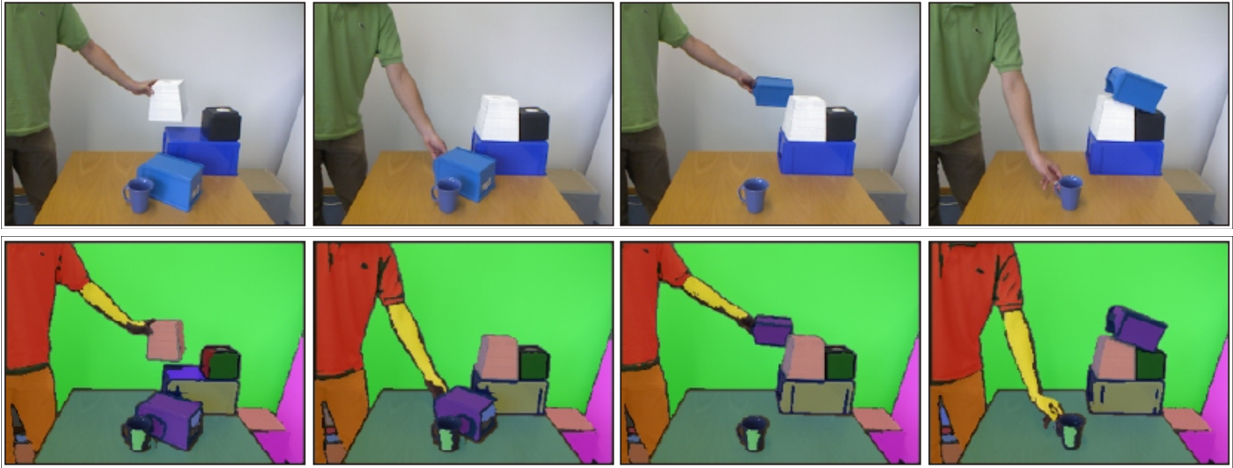
\includegraphics[width=\linewidth]{figures/Introduction/Video_Segmentation.pdf}
\caption[Example of Video Object Segmentation]{Example of Video Object Segmentation - from \cite{Abramov_WACV12}. This shows the goal of \gls{vos} - to extract a dense labeling (labels here are shown as distinct colors) for every frame, maintaining temporal consistency of objects. For many applications it is of vital importance to make the labeling consistent from frame to frame, that is, to maintain object identities.}
\end{figure}

One interesting aspect of video segmentation is that it has the potential to be more accurate than single image segmentation, as it can take advantage of the temporal coherence of objects to infer information about the objects in a scene. Unfortunately, the addition of the temporal domain brings along new challenges as well; for instance that pixels which should be grouped across time may not be continuously visible, as in the case of partial or full occlusions. Additionally, the added dimension increases the computational complexity of the problem, making accurate segmentation a costly procedure. Temporal information also increases the exposure of the algorithm to noise, as each image frame is a separate noisy measurement. This adds a large amount of uncertainty to the problem, since measured values (i.e., of color) for an object can show significant variation over time. 
 
\section{State of the Art}
\subsection{Segmentation and Superpixels}
Segmentation of scenes into objects remains one of the most challenging topics of computer vision despite decades of research. To address this, recent methods often use hierarchies which create a rank order that build bottom-up from small localized superpixels to large-scale regions \cite{Ren:ICCV2003,Ahuja:CVPR2008,Arbelaez:PAMI2011}. As an alternative, researchers have also pursued strictly top-down approaches. Such methods began with coarse segmentations using multiscale sliding window detectors \cite{ViolaJones:IJCV2004}, later progressing to finer grained segmentations and detections based on object parts \cite{Felzenswalb:PAMI2010, Bourdev:ICCV2009}. These two avenues of research led naturally to methods which {\em combine} bottom-up hierarchy building with top-down object- and part-detectors \cite{Arbelaez:CVPR2012, Silberman:ECCV12, Gupta:CVPR2013}. While these approaches have yielded quite good results even on complex, varied data sets, they have lost much of the generality of learning-free approaches. In general the most powerful methods to-date use trained classifiers for segmentation \cite{Silberman:ECCV12, Gupta:CVPR2013}. This means they cannot be applied to arbitrary unknown scenes without being retrained, requiring the acquisition of a new data-set tailored to each test environment and a-priori models specialized to this testing data.

\subsection{Multi-Target Visual Tracking}
\gls{mtvt} is a well-established field, which goes back over thirty years \cite{MTT_JPDA}. In this work we use  Sequential Bayesian Estimation to track targets, in particular a Monte Carlo method known as Particle Filtering. This approach was first introduced to the vision community by Isard and Blake \cite{Condensation98} and has been the subject of much subsequent research extending it \cite{TrackingMultipleParticleFiltering,MonteCarloMTT,SequentialMonteCarloMultitargetFiltering}.

There are two standard approaches that have been used to extend the Particle Filter to multiple targets. The first represents all targets jointly in a single particle filter by assigning individual particles to particular labels \cite{MultiMixtureTracking03}. This means that, for a given total number of particles, there will be fewer for each individual target - resulting in reduced accuracy. The second approach is to add additional dimensions to the state space for each additional target \cite{TrackMultTargets01}. Unfortunately, this approach quickly increases the dimensionality of the state space, which also results in a need for a very high number of particles for the filter to remain accurate. 

In both of the above approaches, the computational complexity increases exponentially as targets are added (for constant level of accuracy). As a consequence of this, it is beneficial to use a separate particle filter for each target. One way of doing this is to add factors to the observation and/or process models of the filters which explicitly model occlusions and interactions between targets \cite{MCMCPartFilt_05, ApproxMultiTrack_06}. Alternatively, one can use a discrete processing step to resolve the association of target detections \cite{Koo_IROS2013}. 

A different approach which has generated much interest is to use the output of detectors as the basis for tracking. Known as \emph{tracking-by-detection}, these methods typically use simple particle filters to maintain tracks \cite{RobustVTMT_06,MultipersonTBD_011}, and shift the focus of the problem onto the data association step, wherein detections are assigned to targets. While there are several classical approaches for solving this association problem from Sonar and Radar research \cite{SonarMultiTrack_83,MultiTrack_79}, a greedy approach is typically sufficient given a good association scoring function \cite{DetTrackMultiHumans_07,MultipersonTBD_011}. 

\subsection{Video Object Segmentation}
There are many existing \gls{vos} methods, which can be classified based on three parameters; whether they are on- or off-line, whether they are dense or sparse, and whether or not they are supervised. We can reduce the comparison-space of related work by comparing only with algorithms which have the same three parameters as this work - on-line processing (the algorithm may only use past data), dense segmentation (every pixel is assigned to a spatio-temporal cluster), and unsupervised operation. Four state-of-the-art segmentation algorithms meet these requirements: \gls{msvs} \cite{MSVS}, \gls{mhvs} from superpixel flows \cite{MHVS}, \gls{pva} of a preceding graph \cite{PropValAgg}, and Matching images under unstable segmentations \cite{MatchingUnstable}.  Of these methods, none are able to handle full occlusions; in fact only \gls{mhvs} considers occlusions, and it is only able to handle partial occlusions for a few frames, and does not consider full occlusions. Even state of the art off-line methods such as that of Brendel and Todorovic \cite{SegTrackRegions} only handle partial occlusions, claiming that ``complete occlusions ... require higher-level reasoning''.  

In \cite{TrackingOcclusionsGraphCuts} Papadakis and Bugeau use a dynamical model to guide successive segmentations, along with an energy function minimized using graph cuts to solve the label association problem. They formally model visible and occluded regions of tracked objects, tracking them as distinct parts. While they do consider occlusions, they do not maintain a world model, and as such their methodology must fail under complete occlusions.  Additionally, they formally model visible and occluded parts of the tracked objects, and so the method does not scale well with an increasing number of objects, and thus is better suited to extracting the silhouettes of a few objects than performing a full segmentation. Other methods, such as \cite{LayeredGraphicalModels}, are severely limited in that they require pre-
computed models which are calibrated to a ground plane in order to resolve occlusions. Recent work in \gls{mtvt}~\cite{MultiObjectTracking} successfully tracks multiple objects using a segmentation and association approach and adaptive 3D appearance models, but is limited by the need to align model point clouds to the observed data every frame, as well as the need for a ground plane. This precludes it from handling occlusions, as once a target is no longer observed, its track must be terminated.

\section{Outline and Contributions}
This work is organized as follows: First, in Chapter \ref{Chap:VideoSegRelaxation} we present a hybrid \gls{vos} / \gls{mtt} technique for 2D data. We describe the segmentation algorithm used, how we track segments, how we combine tracked results into a video segmentation and finally present results on a tracking benchmark. In Chapter \ref{Chap:WorldModel} we present the concept of a persistent 3D voxel world model. We begin by briefly introducing some core concepts of acquisition and representation of 3D point cloud data, then present \gls{vccs}, a method for extracting a graph of 3D voxel patches from point cloud data. We then discuss how to add point clouds sequentially to the model in a way that allows voxels to persist through occlusions. Finally, we present quantitative and qualitative results of \gls{vccs} and \gls{lccp}, a segmentation method which uses \gls{vccs}. In Chapter \ref{Chap:ModelBasedTracking} we describe a method for using particle filters to track multiple rigid objects in point cloud video data and present results of tracking performance on both real and artificial data. Additionally, we present a stratified sampling approach which greatly reduces the computational complexity of tracking. In Chapter \ref{Chap:TrackingBasedSegmentation} we combine the methods described in prior Chapters into a system which can produce full video segmentation of point cloud videos. We show that the system is highly robust to occlusions and noisy data, and present results on the application of semantic understanding and imitation of human actions. Finally, in Chapter \ref{Chap:Conclusions} we discuss the findings and experimental results of this work, possible future work, and conclude.

Each of the Chapters in this thesis contain novel contributions to the field, briefly described below. 
\begin{itemize}
\item {\bf Chapter \ref{Chap:VideoSegRelaxation} } contains a 2D segmentation through relaxation technique published in \cite{PartFilter_Papon_2012}. This work demonstrated the concept of extracting video segmentation from tracks, and the idea of connecting segmentation and tracking in a closed feedback loop.

\item {\bf Chapter \ref{Chap:WorldModel} } contains the Supervoxel clustering method \gls{vccs}, as well as the scheme for maintaining voxels in an octree through occlusions published in \cite{VCCS_Papon_2013}. Supervoxels serve as the basis for much ongoing work, as they provide a graph structure for otherwise unordered pointcloud data.

\item {\bf Chapter \ref{Chap:ModelBasedTracking} } accelerates 3D correspondence particle filter tracking through a stratified sampling of the model-space published in \cite{PaponWACV_2015}. This technique greatly reduces the computational complexity of pointcloud tracking by taking advantage of the spatial structure of points.

\item {\bf Chapter \ref{Chap:TrackingBasedSegmentation} } has the techniques used to generate full segmentations based upon the results from multiple independent trackers \cite{PaponIros2013}. 

\item {\bf Appendix \ref{chap:Oculus} } presents the Oculus Vision System \cite{Oculus_Papon_2012}, an open-source computer vision system created over the course of the research for this thesis.
\end{itemize}

Additionally, the methods presented in this work have all been published as open-source and are publicly available, either as part of Oculus\footnote{\url{https://launchpad.net/oculus/}} or the \gls{pcl}\footnote{\url{http://www.pointclouds.org/}}.
